%%%%%%%%%%%%%%%%%%%%%%%%%%%%%%%%%%%%%%%%%%%%%%%%%%%%%%%%%%%%%%%%%%%%%%%%%%%%%%%%%%%%%%%%%%%%%%%%%%%%%%%%%%%%%%%%%%%%%%%%%%%%%%%%%
\chapter{Basic Principles of Augmented Reality}
\label{cha:basic_principles}

Before diving into the description of this project, one should know what is Augmented Reality. In this chapter, we will try to define Augmented Reality, how it works and how it could be used.

%%%%%%%%%%%%%%%%%%%%%%%%%%%%%%%%%%%%%%%%%%%%%%%%%%%%%%%%%%%%%%%%%%%%%%%%%%%%%%%%%%%%%%%%%%%%%%%%%%%
\section{What is Augmented Reality?}
\label{sec:what_is_ar}

Augmented Reality is a term that is used to describe digital systems that display an artificial visual layer of three- or two-dimensional models upon our natural perception of reality in real-time. It aims at improving or completing our limited way of seeing the real world by presenting artificial elements that would otherwise be hidden to our senses.\\

The most commonly known Augmented Reality application is the weather forecast program on television. In this system, a reporter is acting in a real environment in front of a blue/green screen, but the spectator watching his TV will see the reporter standing in front of an animated map: the content of the background consists of virtual data mapped on a real world object in real-time. This is Augmented Reality. \\

It is during the year 1992 that a Boeing researcher named Tom Caudell first defined "Augmented Reality" in a paper called "Augmented reality: an application of heads-up display technology to manual manufacturing processes" \cite{Cau92}. The term was used to describe a digital system that displays virtual graphics onto a physical reality.\\

Yet the concept of Augmented Reality itself is older than its name, since the first Augmented Reality device was build and presented in a 1968 paper by Ivan Sutherland \cite{Sut68}. The system was designed to track the head position of the user to project before his eyes two-dimensional models in order to create an illusion of three dimensions. It relied on the idea that moving perspective images would appear in three dimensions even without stereo presentation, a principle which is called the "kinetic depth effect". In such a system, the user will perceive the object as three-dimensional only when he moves, otherwise the object will only be seen as planar.\\

It has to be noted that Augmented Reality differs from Virtual Reality. In Virtual Reality, there are no elements of Reality, as much as in Reality there are no elements of Virtuality by definition. In his paper called "Augmented Reality: A Class of Displays on the Reality-Virtuality Continuum" \cite{Mil94}, Milgram defines the Reality-Virtuality Continuum shown in Fig. \ref{fig:milgram_diagram}.

\begin{figure}[ht]
\center
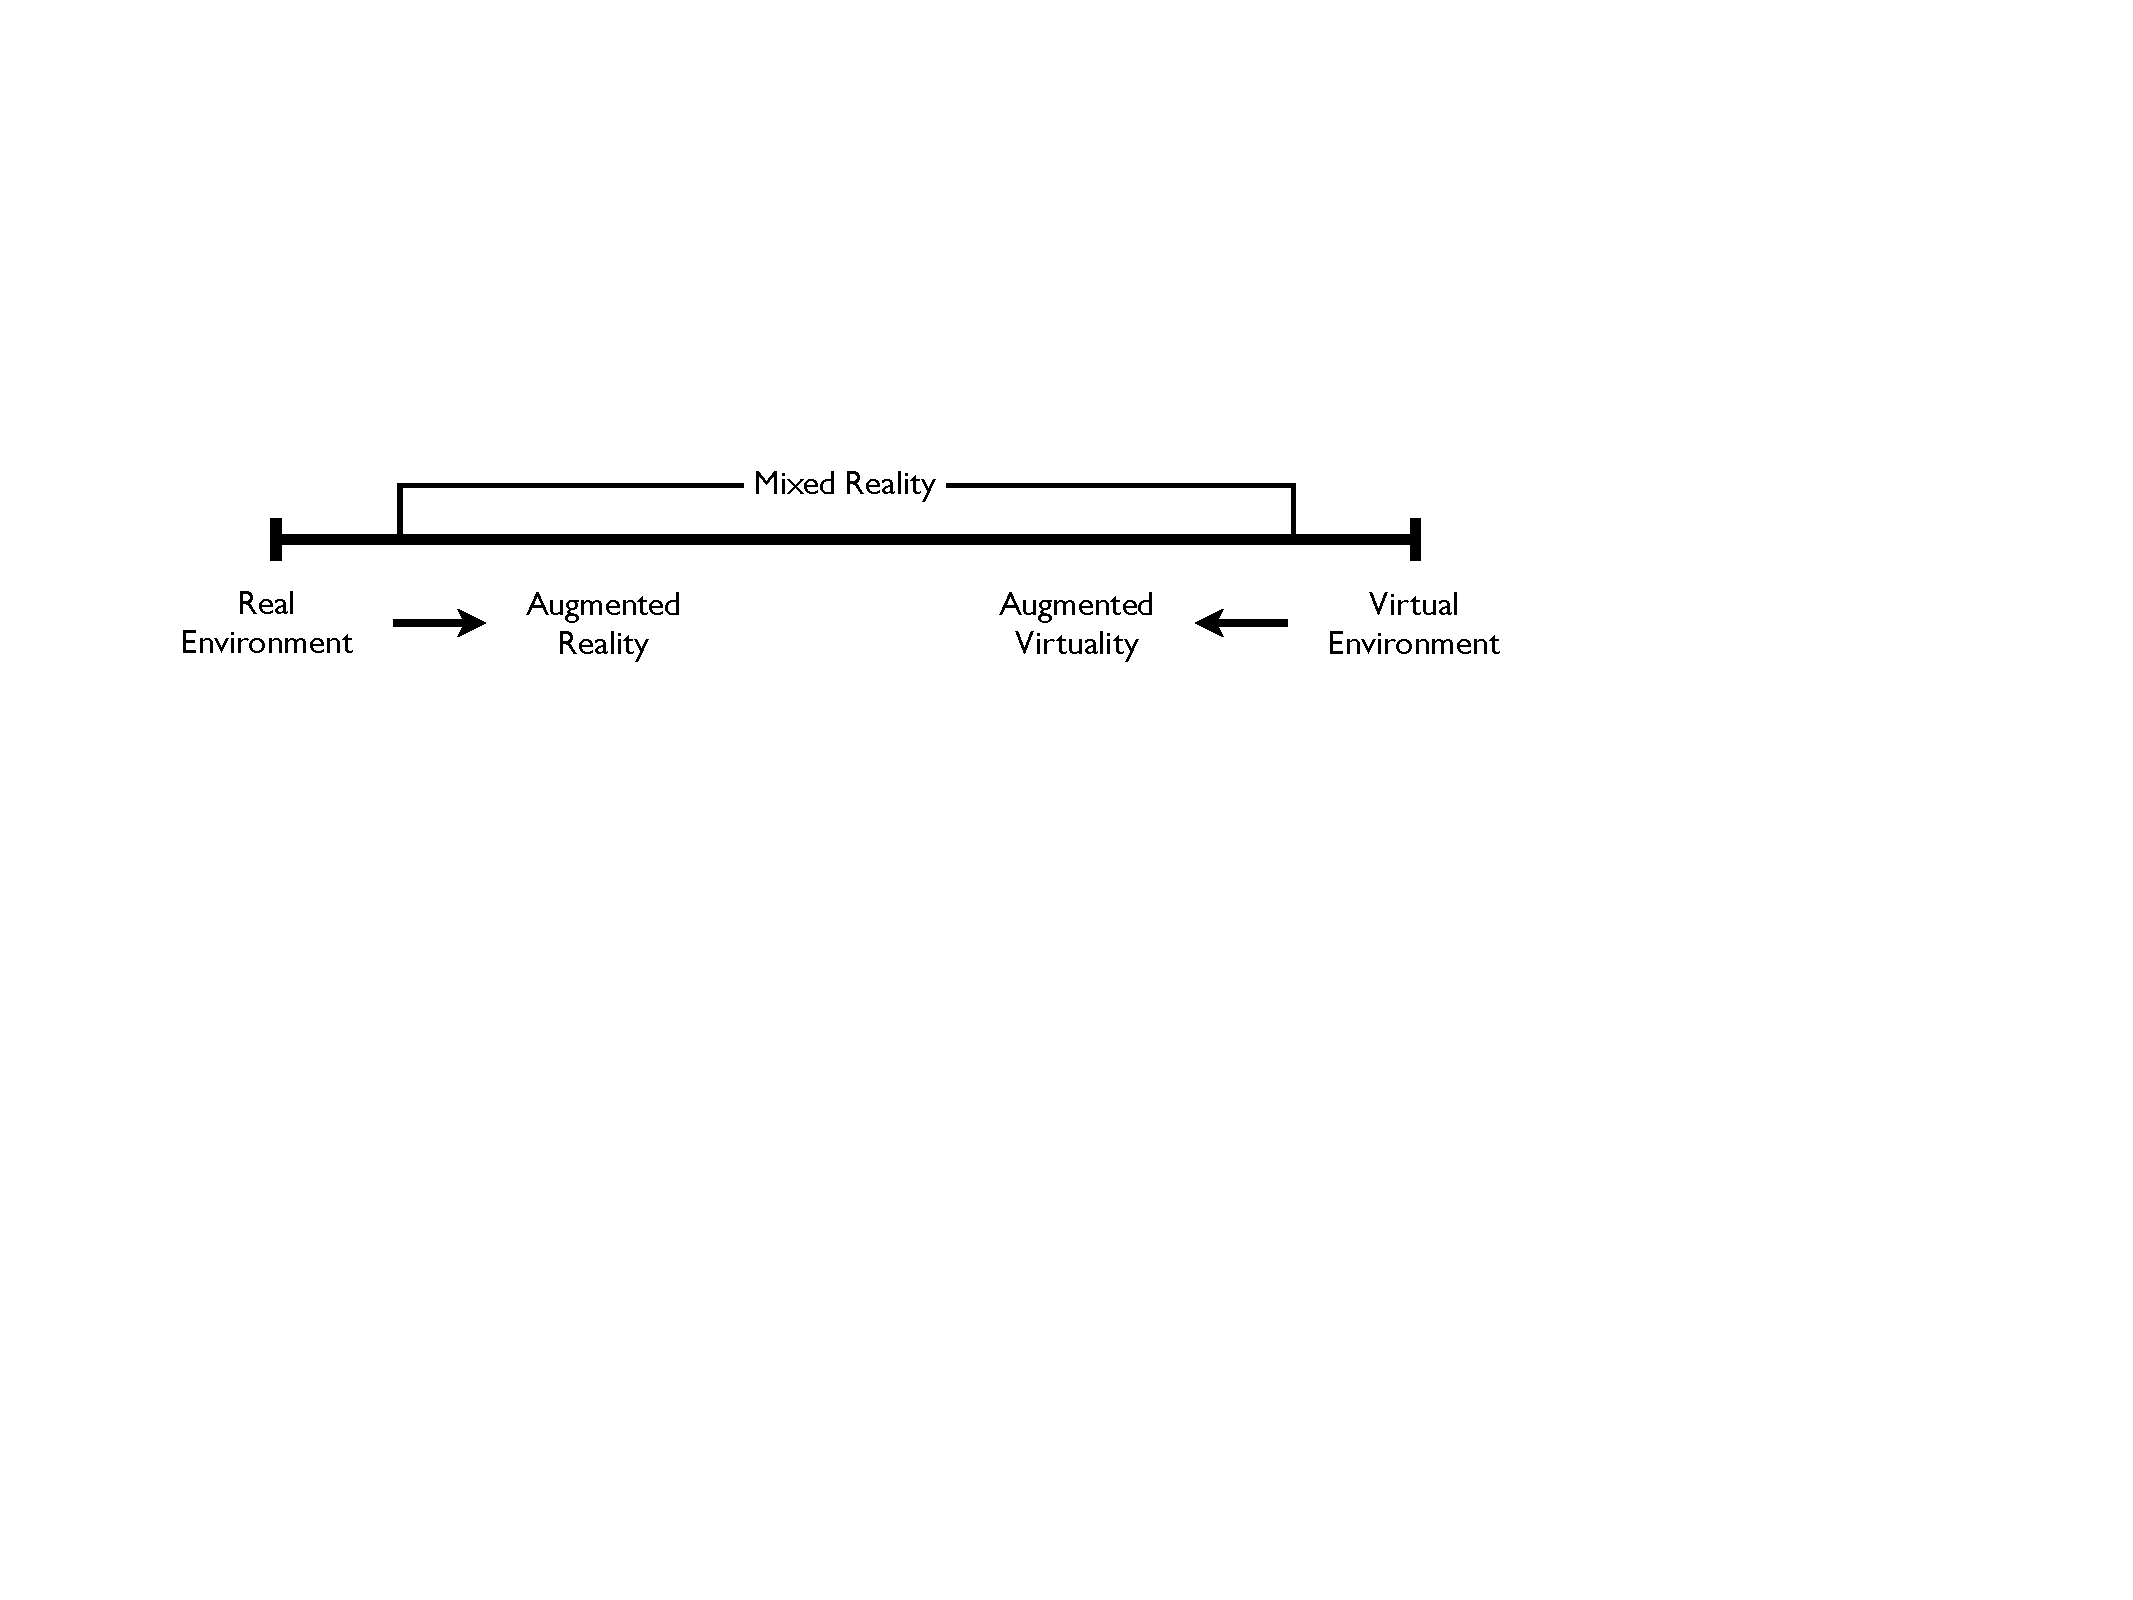
\includegraphics[scale=0.5]{pics/milgram_diagram}
\caption{Milgram's Reality-Virtuality Continuum \cite{Mil94}}
\label{fig:milgram_diagram}
\end{figure}

As can be seen from this diagram, Augmented Reality is based upon reality and tends to Virtuality in an area called "Mixed Reality". It lies near the real world end of the line, which means the predominate perception is the real world. On the symmetric position, Milgram defines Augmented Virtuality. Behind this concept lie systems where real world items are added to a Virtual Environment, such as texture mapping on virtual objects in video games.\\

So the limits of Augmented Reality are defined by the furthest one can go at adding virtual data on a real world representation without depriving the user of its predominate perception of Reality.

%%%%%%%%%%%%%%%%%%%%%%%%%%%%%%%%%%%%%%%%%%%%%%%%%%%%%%%%%%%%%%%%%%%%%%%%%%%%%%%%%%%%%%%%%%%%%%%%%%%
\section{How does it work?}
\label{sec:how_does_ar_work}

In order to get an Augmented Reality application, one must integrate artificial objects into a real scene. Of course, such objects must be rendered to scale and at the correct position and orientation. To do so, the system requires to know the position of the camera or the user from the object. This is the core principle of Augmented Reality.\\

To solve this problem, there are two main approaches:

\begin{itemize}
\item{Use sensors to know the position of the object from the camera}
\end{itemize}

By the mean of tags on a real object, one can get a coordinate system on which to project a virtual model. Those tags can be visual or based on any technology that can be use to locate that object, for example a set of Infra-Red diodes.

\begin{itemize}
\item{Use sensors to know the position of the camera in a known space}
\end{itemize}

If the environment is known, i.e. the application is internally aware of the position of the object, or if the object is fully virtual and does not rely on any physical counterpart, one can evaluate the position of the camera in this environment and render the object accordingly. The position of the camera can be known by the mean of a large enough set of sensors that will be able to position it in the environment space.\\

Once the virtual environment is known, each virtual object must be rendered on top of an existing view by the mean of geometric projections that fit the estimated position of this object in the virtual space. The virtual object can also be projected onto a real world object such as a screen or an holographic system.

%%%%%%%%%%%%%%%%%%%%%%%%%%%%%%%%%%%%%%%%%%%%%%%%%%%%%%%%%%%%%%%%%%%%%%%%%%%%%%%%%%%%%%%%%%%%%%%%%%%
\section{What is it for?}
\label{sec:what_is_ar_for}

Augmented Reality has been used in domains where the purely visible environment is not sufficient or satisfactory and has to be completed by additional information in a non-obstructive way. One of the first application was in head-up displays for military aircraft as shown in Figure \ref{fig:headup_display}.\\

\begin{figure}[ht]
\center
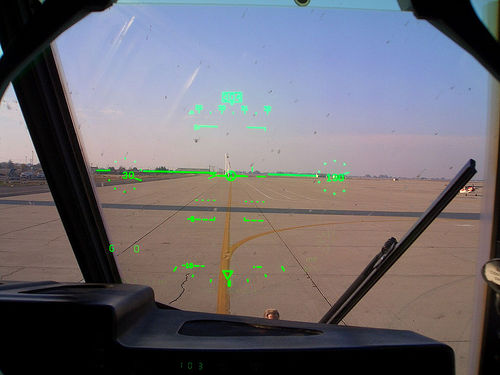
\includegraphics[scale=0.6]{pics/headup_display}
\caption{An Head-up display in a military plane \cite{headupsource}}
\label{fig:headup_display}
\end{figure}

Many applications have also been developed for surgery and medical imagery, presenting serious advantages over non-assisted methods.\\

But nowadays, we also see appearing more casual applications, especially for marketing purposes.\\

In a recent web publication \cite{Hay09}, an interesting study on an Augmented Reality business model has been proposed by Gary Hayes. In his study, he tries to categorize all the exploitable applications of Augmented Reality. Figure \ref{fig:AR_business_model} shows an attempt at classifying the different approaches at Augmented Reality applications according to their potential as marketable products.\\

\begin{figure}[ht]
\center
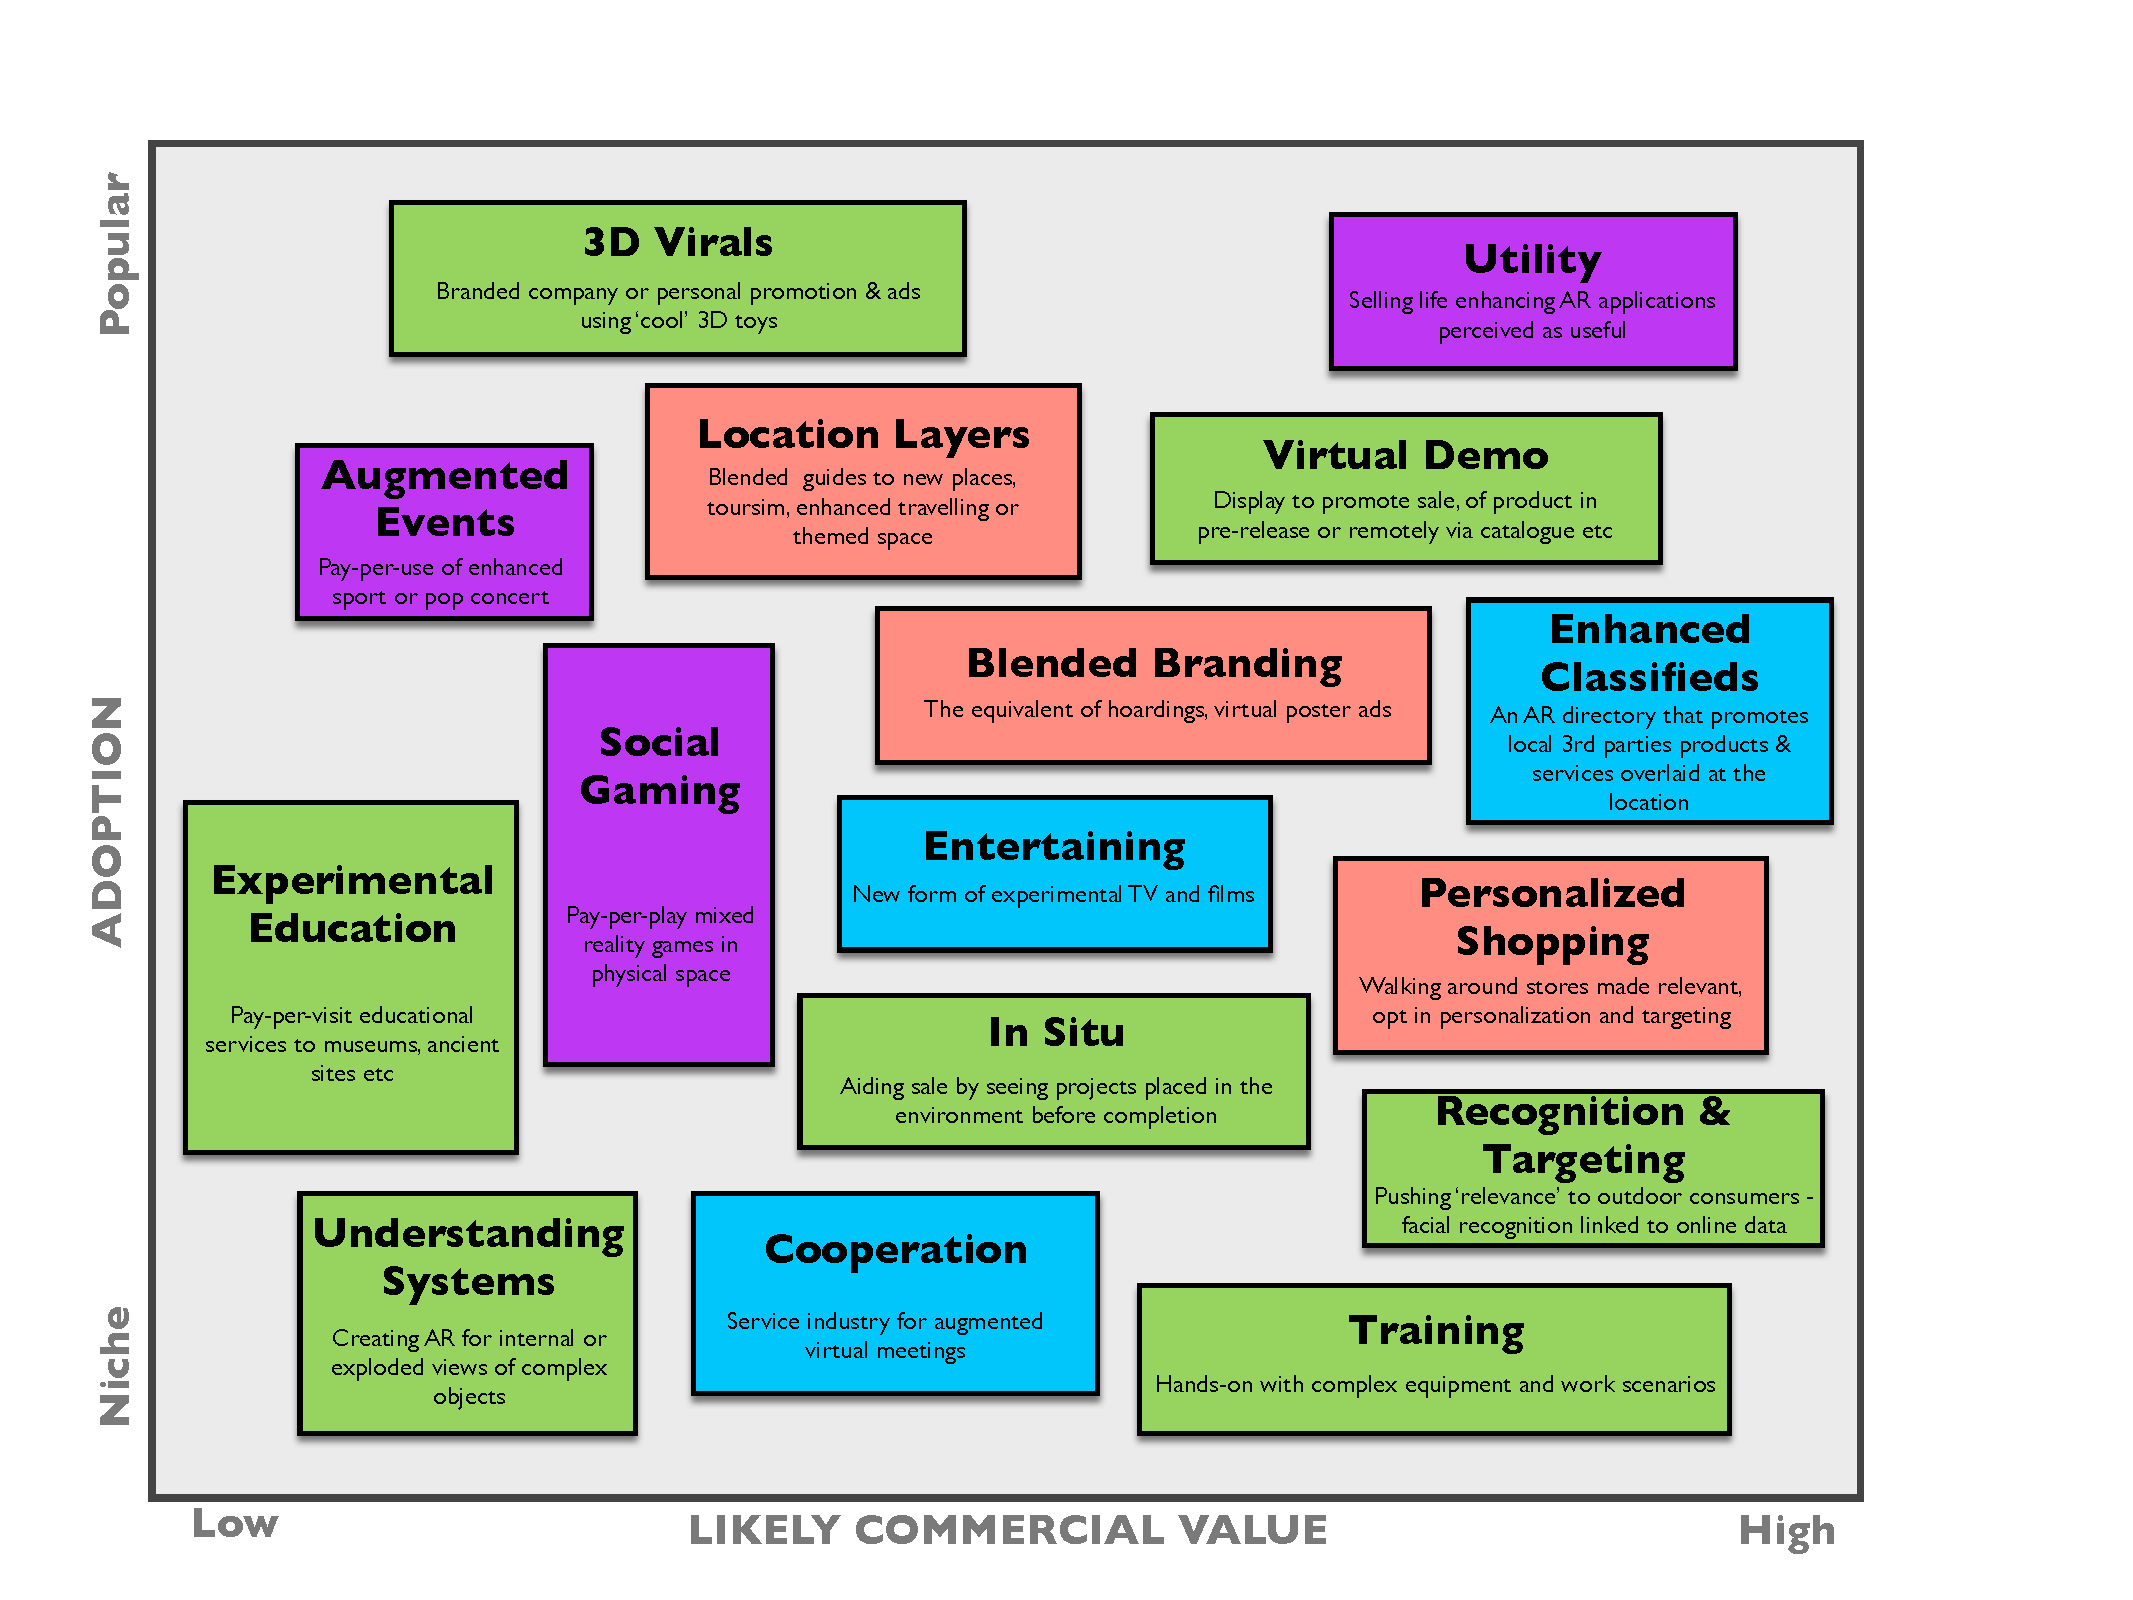
\includegraphics[scale=0.4]{pics/AR_business_model}
\caption{16 Augmented Reality Business Models by Gary Hayes \cite{Hay09}}
\label{fig:AR_business_model}
\end{figure}

In this thesis, we tried to fit into the "Utility" business model, being the most promising one according to this analyse (popular and high likely commercial value).\\

